\chapter{Rețelistică}
\vskip -25pt
\textit{Cu PHP controlezi ce se întâmplă pe server,\footnote{În acest
capitol vei vedea că termenul {\glqq}server{\grqq} este deseori folosit greșit,
ca și în acest paragraf.} server care
este conectat la Internet.
Deci folosirea PHP este strâns legată
de rețea. Din acest motiv, înțelegerea noțiunilor fundamentale de
rețelistică este indispensabilă.\footnote{De exemplu pentru 
înțelegerea implicațiilor de securitate, folosirea extensiilor
precum \textsl{cURL} sau cereri asincrone -- \textsl{AJAX}. Nu îţi face griji dacă
nu înţelegi toţi aceşti termeni deocamdată.}
Nu voi intra în toate detaliile, doar în ce ai nevoie ca programator
și pentru a-ți seta mediul de programare în PHP, pentru a crea
\textsl{website}-uri sigure, și pentru a înțelege noțiunile
necesare în folosirea extensiilor PHP care lucrează cu rețeaua.
}

\vskip 5em

\section{Noduri, TCP/IP, rețele}
\engl{Rețelistica}{networking} se ocupă cu comunicarea între
așa-zise \engl{noduri}{nodes}. Un nod poate fi un calculator
personal, un router, un server, practic orice dispozitiv digital
conectat la reţea.

Înainte de a vedea printr-un exemplu practic prin ce noduri
din rețea trec informațiile
atunci când cauți ceva pe \textsl{web} cu google, trebuie să faci
cunoștință cu câteva definiții generale.

Există două mari tipuri de interfețe pentru interacțiunea cu un 
\engl{sistem de operare}{operating system}\footnote{abv. OS}:
%TODO adăugare index termeni şi abreviatii

\begin{itemize}
	\begin{item} \engl{\href{http://en.wikipedia.org/wiki/Graphical_user_interface}{GUI}}{graphical user interface}
	\begin{description}
	\item Este cea mai comună printre utilizatorii ocazionali, este ușor de utilizat
	și nu necesită cunoștințe avansate de IT pentru a o folosi. Însă te
	limitează în folosirea programelor
	\end{description}
	\end{item}
	
	\begin{item}
	\engl{\href{http://en.wikipedia.org/wiki/Command-line_interface}{CLI}}{command line interface}
	\begin{description}
	\item Este destinată profesioniștilor. Necesită
	cunoștințe mai avansate, însă este mult mai puternică și flexibilă
	\end{description}
	\end{item}
\end{itemize}
Sub MS Windows, interfața CLI este cunoscută și ca \textsl{MS-DOS Prompt}. Pentru
a-l lansa în execuție, du-te în \texttt{Start -> Run}, și tastează \texttt{cmd}.
Apare o fereastră neagră și neprietenoasă. Sub GNU/Linux aceasta este
cunoscută sub numele de \textsl{consolă}, \textsl{terminal} sau
\textsl{shell} (unul dintre ele fiind \textsl{bash}).

Deschide interfața CLI a sistemului tău și introdu comanda
\texttt{tracert google.com} pentru Windows sau \texttt{traceroute google.com} pentru 
GNU/Linux. Figura \ref{fig:cli traceroute} îţi dă un exemplu de \textsl{output}.

\begin{figure}[h!]
  \centering
    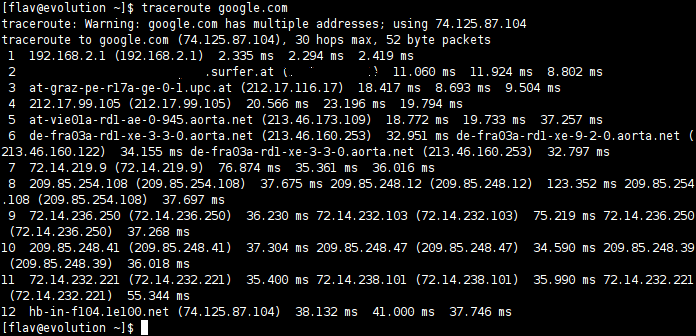
\includegraphics[width=300px]{cap01/traceroute.png}
  \caption{Ruta către un nod}
  \label{fig:cli traceroute}
\end{figure}

După cum vezi, tot ceea ce îi trimit eu lui google.com și ce îmi trimite
el înapoi trece prin alte 11 noduri din rețea. Dacă un \engl{infractor}{cracker}
deține controlul asupra unuia dintre aceste noduri,
poate vedea absolut orice {\glqq}vorbesc{\grqq} eu cu \texttt{google.com}. Un astfel de atac
se numește \href{http://en.wikipedia.org/wiki/Man-in-the-middle_attack}{man in the middle},
deoarece atacatorul se află la mijloc, între
cele două \engl{capete}{endpoints}.

Bineînțeles că nu numai eu aș fi
victima unui astfel de atacator, ci oricine trimite \engl{pachete de date}{data packets}
oricui altcuiva (nu neapărat numai lui \texttt{google.com}), atâta timp cât pachetele
de date trec prin nodul controlat de el.

Toate nodurile din reţeaua globală numită Internet au o adresă unică numită adresă
\engl{IP}{internet protocol}. Ea este de forma \texttt{xxx.xxx.xxx.xxx}, unde \texttt{xxx} este un număr
între 0 şi 255. Unele adrese IP au o semnificaţie specială. De exemplu, fiecare
nod are adresa IP \texttt{127.0.0.1}. Ea nu este utilă în Internet, deoarece orice pachet
de date trimis la acea adresă ajunge înapoi la expeditor, fără nici măcar a trece
pragul sistemului local. Încearcă de exemplu comanda \texttt{tracert 127.0.0.1}.

Alt bloc de adrese IP speciale sunt toate adresele între \texttt{192.168.0.0} şi
\texttt{192.168.255.255}. Ele sunt rezervate \engl{reţelelor locale}{local area network}.\footnote{abv. LAN}

Un astfel de exemplu este chiar reţeaua mea
locală\footnote{Un bun punct de start este \url{http://en.wikipedia.org/wiki/Private_network}.
De acolo poţi urma link-uri intersante către noţiunile ce urmează a fi introduse,
şi multe alte lucruri neprezentate aici.}.
După cum vezi în figura \ref{fig:cli traceroute},
pachetele de date care pleacă de la mine trec mai întâi prin nodul \texttt{192.168.2.1}.
Aceasta este adresa \textsl{router}-ului\footnote{\url{http://en.wikipedia.org/wiki/Router}}
meu. \textsl{Topologia} reţelei din perspectiva mea
arată ca în figura \ref{fig:topologie}.

\begin{figure}[h]
  \centering
    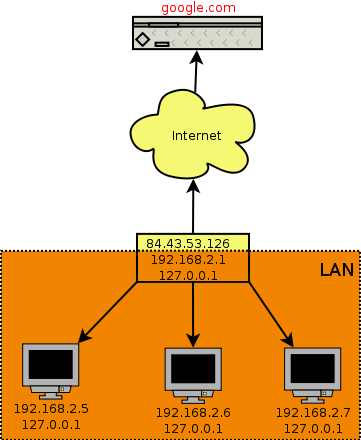
\includegraphics[width=100px]{cap01/Diagram1.png}
  \caption{Exemplu de topologie a unui LAN}
  \label{fig:topologie}
\end{figure}

Misiunea unui \textsl{router} este să distribuie pachetele
pe care le primeşte altor calculatoare din \textsl{LAN}-ul meu. Asta îmi permite să am acces
la Internet cu mai multe calculatoare, însă din exterior \textsl{LAN}-ul este văzut ca
având o singură adresă IP: \texttt{84.43.53.126}, şi deci ca un singur calculator. Dacă
nu puneam acest \textsl{router} între calculatoarele mele şi Internet, nu puteam conecta
la Internet decât un singur calculator, care avea adresa IP \texttt{84.43.53.126}.

\sloppy Există deci două tipuri de adrese IP, cele interne reţelei mele, precum \texttt{192.168.2.1}
sau \texttt{192.168.2.6} şi cele externe reţelei, publice, precum \texttt{84.43.53.126} sau una
dintre adresele lui \texttt{google.com}, \texttt{74.125.87.104}.
Cele dintâi se numesc \textsl{adrese private}\footnote{le poţi numi şi {\glqq}intranet{\grqq},
analog cu cele publice, {\glqq}internet{\grqq}.}
sau adrese LAN, cele din urmă sunt în schimb \textsl{adrese publice}.

\attention{Internetul este o reţea de LAN-uri şi \engl{WAN-uri}{wide area network} interconectate.
Asta transformă Internetul în cea mai mare WAN, o reţea globală.}

Dacă nu ai un \textsl{router} la mijloc, între tine şi Internet, atunci îţi poţi vedea adresa IP
externă prin interfaţa pusă la dispoziţie de sistemul tău de operare. Sub windows, introdu
comanda \texttt{ipconfig /all} în CLI, sub GNU/Linux \texttt{ifconfig -a}.

Dacă însă ai un router la mijloc, şi nu ştii cum să-i accesezi interfaţa de configurare,
atunci trebuie să îi ceri unui alt calculator de pe Internet să-ţi spună ce adresă IP
vede el că ai, pentru că ce vede el va fi mereu adresa ta Internet, externă.

\begin{Exercise}[title={What is my IP Address?},difficulty=1]
Caută pe web cu un motor de căutare \textit{what is my ip address} şi compară
adresa afişată de acea aplicaţie web cu ce adresă IP îţi raportează OS-ul tău.
%Din această comparaţie vei deduce dacă între tine şi Internet se află un router sau dacă eşti conectat direct la Internet.
Ce poţi deduce din această comparaţie?
\end{Exercise}

\section{Domenii}
Teoretic, este suficient să ştii adresa IP a unui nod pentru a comunica cu el. De exemplu,
am aflat că una dintre adresele IP ale lui \texttt{google.com} este 74.125.87.104. Deci putem
intra bine mersi pe adresa \texttt{http://74.125.87.104}.

Însă oamenii nu pot reţine uşor numere. De aceea s-a inventat \engl{DNS}{domain name system},
un sistem care converteşte nume precum \texttt{google.com}, în adrese IP. Atunci când introduci
\texttt{google.com} în browserul tău, acesta trimite o cerere la serverul DNS şi primeşte
înapoi adresele IP asociate cu \texttt{google.com}. Abia apoi se conectează la acea adresă IP,
şi îi cere informaţii.

Sub MS Windows îţi poţi afla serverele DNS cu aceeaşi comandă \texttt{ipconfig} şi parametrul
\texttt{/all}. Sub GNU/Linux, acestea se află în mod normal în fişierul \texttt{/etc/resolv.conf}.

Să presupunem că serverele tale DNS se deconectează de la reţea.\footnote{O glumă
comună este să spui că administratorul serverului s-a împiedicat din greşeală de stecher
şi l-a tras din priză fără să îşi dea seama.} Atunci nu vei mai putea accesa \texttt{http://google.com},
pentru că browserul tău nu mai poate afla adresa IP corespunzătoare. Însă asta nu te împiedică
să introduci manual adresa IP, dacă o ştii.

Pentru a afla dacă un nod este conectat la reţea se foloseşte comanda
\texttt{ping}\footnote{o numim comandă, însă în realitate este un program,
şi se numeşte \texttt{ping.exe}}, având primul
parametru adresa IP pe care vrei să o verifici.

\begin{Exercise}[title={Ping your DNS server}]
Află adresa IP a serverului tău DNS şi trimite-i un pachet de date cu \texttt{ping}.\footnote{Acest exerciţiu nu trebuie
rezolvat în cadrul programului de tutelare, este un exerciţiu suplimentar,
pentru tine.}
\end{Exercise}

Poţi interoga manual serverul DNS cu comanda \texttt{nslookup}
(en. \textsl{nameserver lookup}). Exemple:
\texttt{nslookup google.com}, \texttt{nslookup 192.0.32.10}.
Este deci posibil să afli atât adresele IP pornind de la un nume precum
\texttt{google.com}, însă şi numele, pornind de la o adresă IP de Internet
(nu de intranet).
Deşi este posibil ca mai multe domenii să \textsl{pointeze} către aceeaşi
adresă IP, o adresă IP nu poate {\glqq}pointa{\grqq} (prin \textsl{reverse DNS})
decât spre un domeniu.\footnote{Tehnic este posibil, însă practic poate
cauza probleme.}

Totuşi, din ce este compusă o adresă precum \texttt{www.google.com}?
\texttt{.com} se numeşte \engl{TLD}{top level domain}. Ceea ce se află în stânga
sa este un \textsl{subdomeniu}, până la următorul punct.
Astfel, \texttt{google} este un subdomeniu al lui \texttt{.com},
iar \texttt{www} este un subdomeniu al lui \texttt{.google.com}.

Dacă vrei să ai un domeniu al tău, trebuie să cumperi unul de la
o firmă numită \href{http://en.wikipedia.org/wiki/Domain_name_registrar}{domain name
registrar}. Pentru a învăţa PHP nu ai nevoie de un domeniu, poţi
face totul pe calculatorul tău personal, aşa cum vei vedea în acest capitol.

\section{Protocoale}
Internetul este {\glqq}făcut{\grqq} din aşa-numite \textsl{servicii}. Cele mai cunoscute servicii sunt
web-ul pentru documente interconectate,\footnote{Prin link-uri.}
\textsl{pop3} sau \textsl{imap} pentru e-mail,
\textsl{irc} (en. \textsl{internet relay chat}) pentru chat, sau
\textsl{ftp} (en. \textsl{file transfer protocol}) pentru transferul de fişiere.

Pentru a folosi unul dintre aceste servicii, ai nevoie de un program
special numit \textsl{client}. Nu există un client care să {\glqq}ştie{\grqq} 
să acceseze toate serviciile, pentru
că fiecare serviciu este diferit de celelalte. Vom vedea mai târziu de ce.

Astfel, avem clienţi pentru www, clienţi pentru ftp, clienţi pentru irc, ş.a.m.d.

Serviciul \textit{world wide web}, sau pe scurt \textit{web}-ul, este atât de răspândit, încât
oamenii au dat un nume special clienţilor www: \textsl{browser}. Există mai multe browsere,
create de diferite firme. Printre cele mai cunoscute se numără:
\begin{itemize}
\item \href{http://en.wikipedia.org/wiki/Firefox}{Firefox}, creat de Mozilla
\item \href{http://en.wikipedia.org/wiki/Internet_explorer}{Internet Explorer}, creat de Microsoft
\item \href{http://en.wikipedia.org/wiki/Opera_(web_browser)}{Opera}, creat de Opera Software
\item \href{http://en.wikipedia.org/wiki/Chrome_(web_browser)}{Google Chrome}, creat de Google
\item \href{http://en.wikipedia.org/wiki/Safari_(browser)}{Safari}, creat de Apple
\end{itemize}

Colocvial vorbind, te poţi referi la client şi
ca fiind calculatorul pe care rulează clientul, sau chiar la utilizatorul uman din spate
care îi dă instrucţii clientului. În explicaţii voi încerca să nu mă exprim colocvial, ci
corect din punct de vedere tehnic.

În continuare vom clarifica ce se întâmplă atunci când ceri o pagină web cu ajutorul
unui browser de la un server.

Imaginează-ţi că un calculator stă conectat la reţea şi
nu face nimic din {\glqq}proprie iniţiativă{\grqq}.
Acest calculator se numeşte \textsl{server}. Pe server, care este
\textit{maşina fizică}, rulează \textit{un program} numit \textsl{daemon}.
Acesta aşteaptă conexiuni din
exterior, pe care să le deservească. Administratorul serverului va spune colocvial
\textit{the server is up and running}, dar ce vrea să spună de fapt este că \textit{serverul
este conectat la Internet iar cel puţin un daemon aşteaptă noi conexiuni}.

Să nu uităm că fiecare serviciu este diferit. Aşa cum avem diferiţi clienţi pentru
diferite servicii, tot la fel avem şi \textit{daemon}-uri diferite pentru fiecare serviciu.

Exemple de astfel de \textit{daemon}-uri: \textsl{apache} pentru serviciul
www, \textsl{UnrealIRCd} pentru irc,
\textsl{postfix} pentru e-mail, ş.a.m.d. Reţine că acestea sunt programe, la fel
cum este şi \texttt{firefox.exe}. În contrast cu asta noţiunile de \textit{client} şi
\textit{daemon} sunt clasificări
generice pentru tipuri de software.

Ceea ce nu am încetat să sugerez până acum devine evident: cele două părţi, clientul
serviciului pe care doresc să-l utilizez, şi daemonul care e capabil să-i răspundă
clientului meu cu informaţii utile, trebuie să comunice unul cu celălalt.

Această comunicare dintre cele două programe se va desfăşura într-un limbaj comun numit
\textsl{protocol}. Fiecare serviciu are un protocol specific lui. Astfel avem un
protocol irc pentru serviciul irc, protocolul ftp pentru serviciul ftp,
sau protocolul http pentru serviciul web, ș.a.m.d. De aici vine acel {\glqq}http://{\grqq} care precede
orice adresă web. Această adresă se numeşte
\engl{\href{http://en.wikipedia.org/wiki/Uniform_Resource_Locator}{URL}}{uniform resource locator},
o formă de \engl{\href{http://en.wikipedia.org/wiki/Uniform_Resource_Identifier}{URI}}{uniform resource identifier}.

De obicei pe un server rulează mai multe \textit{daemon}-uri în paralel şi care
aşteaptă să deservească cereri. Dar cum să ştie sistemul de operare al serverului
pentru ce daemon este destinat un anumit pachet de date? Din câte ştim până acum,
nu are cum, pentru că OS-ul nu înţelege noţiunea de {\glqq}protocol{\grqq}. Totuşi OS-ul trebuie
să paseze datele primite pachet cu pachet daemon-ului corect.

Pentru a rezolva această problemă fiecare pachet de date este {\glqq}însemnat{\grqq} cu un \textsl{port}.
Un port este un număr între 1 şi 65535 care îi permite sistemului de operare să
paseze pachetul de date procesului\footnote{Un program care este executat. Gândeşte-te
la ce listează {\glqq}task manager{\grqq}.} corect.

Atunci când \engl{administratorul serverului}{sysadmin} lansează în execuţie un daemon,
acesta îi spune OS-ului că \engl{ascultă}{listen}
pe un anumit port. Din acel moment, OS-ul
{\glqq}ştie{\grqq} că acel port îi {\glqq}aparţine{\grqq} acelui daemon. Astfel, sysadmin-ul poate rula
pe sistemul său mai mulţi daemoni concomitent, chiar şi pentru servicii diferite, fără
a-şi face griji că pachetele de date ar putea ajunge la daemon-urile greşite.

Important de menţionat este şi că fiecare serviciu are un port standard. Serviciul www
are 80 ca port standard. Astfel, URL-urile \texttt{http://example.com:80} şi
\texttt{http://example.com} sunt absolut echivalente.

În toate cele explicate până acum nu am intrat în detalii importante precum
\href{http://en.wikipedia.org/wiki/Internet_Protocol_Suite}{TCP/IP}, însă este recomandată citirea şi
înţelegerea acelor noţiuni, cât şi a celorlalte articole pe care le poţi urma de acolo.
Foarte importantă este şi înţelegerea modelului
\engl{\href{http://en.wikipedia.org/wiki/OSI_model}{OSI}}{open system
interconnection}.

\subsection{Primul exerciţiu de hacking}

Înainte de a trece la conţinutul propriu-zis, vreau să clarific de ce această secţiune
foloseşte termenul \textsl{hacking}.

În primul rând, pentru a face acest capitol mai
atractiv pentru toţi cititorii care s-au plictisit de teoria uscată\footnote{Trebuie să
recunoaştem că nu a fost deloc uscată.} de reţelistică
prezentată până acum,
când ei vor de fapt să înveţe PHP. Nu este ceva iluzoriu, ceea ce vei face în continuare
chiar are de-a face cu hacking. Însă hacking implică mult mai multe\footnote{Şi când
spun asta, nu exagerez.}
 cunoştinţe -- paginile
anterioare doar ţi-au prezentat sumar nişte concepte de bază.

În al doilea rând, pentru a-mi crea ocazia de a explica termenul de hacker.
În zilele noastre, \textsl{mass-media}, în încercarea sa de a crea\footnote{În
sensul de {\glqq}a inventa{\grqq}} senzaţionalul,
a redefinit \textsl{hacker} ca \textit{infractor}. Însă nu asta este semnificaţia
originală a cuvântului. Un hacker este o persoană care înţelege foarte bine ce
face. Poţi fi un hacker în orice domeniu, dar atunci când devii un hacker într-un domeniu,
ştii tot ce mişcă în branşa ta. Un hacker în calculatoare ştie totul despre calculatoare,
începând de la electronica procesorului, şi terminând cu analiza psihologică a
omului în relaţia sa cu
calculatorul (sau, pe larg, cu tehnologia în general).\footnote{Cel mai renumit exemplu este
\href{http://en.wikipedia.org/wiki/Kevin_Mitnick}{Kevin Mitnick}}

O altă concepţie greşită despre hacking este că înseamnă să intri în sisteme care nu-ţi
aparţin (\textit{să le spargi}). Nu asta caracterizează hackerul, ci după cum am mai spus,
înţelegerea lucrurilor cu care are de-a face. Te poţi numi hacker la fel de bine
dacă personalizezi un program scris de altcineva pentru nevoile tale. În astfel
de cazuri se spune că \textsl{ai hack-uit codul sursă}, că l-ai înţeles mai întâi, pentru
a-l putea modifica. După cum vezi, hacking înseamnă \textit{înţelegere}.

Felul în care aplici această înţelegere depinde de tine. Asta nu îi absolvă pe
cei care folosesc ceea ce ştiu pentru lucruri ilegale să fie catalogaţi
drept infractori. Pe de cealaltă parte, hackerii adevăraţi reacţionează acid
când sunt priviţi ca nişte infractori, deoarece ei
ştiu că \textsl{hacking} este de fapt ceva constructiv şi benefic unei minţi sănătoase.
Ei preferă ca infractorii să fie numiţi \textsl{crackeri}, pentru a deosebi binele
de rău.

\vspace{1em}\dotfill\vspace{1em}

Atunci când introduci un URL într-un browser, acesta face multe lucruri în fundal.
Unul dintre cele mai importante lucruri este comunicarea în limbajul
\engl{HTTP}{hyper text transfer protocol} cu \textit{daemon}-ul de pe serverul dorit,
asta după ce a aflat adresa IP a acestuia de la serverul DNS.

Noi vrem să facem manual ceea ce ar face un browser automat pentru noi. Pentru asta,
avem nevoie de un program numit \texttt{telnet}. Este un program foarte simplu, tot ce
face este să stabilească o \textsl{conexiune} cu daemonul, şi să-i transmită datele pe care
le tastăm.

O dată ce conexiunea este stabilită, ambele endpoints (daemonul şi noi, cu ajutorul
clientului telnet) pot scrie la grămadă date. De exemplu dacă noi scriem
\begin{verbatim}
foo
\end{verbatim}
şi daemonul ne răspunde cu
\begin{verbatim}
bar
\end{verbatim}
atunci toate datele comunicate arată ca un fişier cu conţinutul:
\begin{verbatim}
foo
bar
\end{verbatim}

Imaginează-ţi că două endpoints comunică prin plicuri.
Programul care iniţiază conexiunea (numit client), scrie datele pe
care urmează să le trimită într-un plic.

Dacă clientul şi daemonul doar schimbă date {\glqq}aşa cum sunt{\grqq},
aşa cum am face cu telnet, atunci doar acest plic este necesar.
Însă dacă aplicaţiile vor să se înţeleagă reciproc,
ele trebuie să folosească un protocol de comunicare.
Pentru web, acest protocol este HTTP.

Acest protocol de comunicare constituie \textit{layer}-ul \textsl{application level}
din \href{http://en.wikipedia.org/wiki/OSI_model}{modelul OSI}.\footnote{\url{http://en.wikipedia.org/wiki/OSI_model}}

În astfel de cazuri, clientul va trebui să pună în plicul nostru încă
un plic\footnote{sau mai multe, în funcţie de protocolul de comunicare folosit}
cu datele structurate specifice protocolului folosit,
în cazul nostru cele specifice protocolului HTTP.

Majoritatea sistemelor de operare moderne vin cu programul telnet preinstalat.
Deci deschide interfaţa CLI şi lansează programul, pasându-i ca prim parametru numele
serverului, şi \textit{port}-ul ca al doilea parametru, deci:
\begin{alltt}
telnet example.org 80
\end{alltt}
După ce s-a conectat, îi poţi cere daemonului ce document vrei, însă trebuie
să o faci în limbajul HTTP, altfel nu va {\glqq}înţelege{\grqq} ce vrem de la el.
Altfel spus, folosind analogia cu plicul, noi ca oameni, deoarece
ştim că vrem să comunicăm în HTTP, şi deoarece telnet nu are noţiunea
de \textit{application layer}, avem responsabilitatea de a ne
{\glqq}împacheta{\grqq} singuri cererea în încă un plic cu formatul specific HTTP,
plic pe care i-l pasăm lui telnet, care ne va pune plicul
pe rând în toate celelalte \textit{layere} ({\glqq}plicuri{\grqq}) din modelul OSI aflate
sub \textit{application layer}: presentation, session, transport, network, iar
electronica (de exemplu placa de reţea) se va ocupa de data link layer şi
physical layer.\footnote{Lucrurile sunt mult mai complexe, telnet
singur nu ar putea face astfel de lucruri fără susţinere
din partea sistemului de operare. Aici am simplificat imaginea
pentru o mai uşoară înţelegere.}

De exemplu, îi vom cere
pagina de start:
\begin{alltt}
GET / HTTP/1.1\Return
Host: example.org\Return
\Return
\end{alltt}
\attention{Simbolul \Return înseamnă că trebuie să apeşi tasta \keystroke{enter}. Deci pentru a
termina cererea HTTP, apeşi de două ori \keystroke{enter} la rând.
Este posibil ca programul tău telnet să nu afişeze ce tastezi. În acest
caz, trebuie să scrii orbeşte, şi să o faci exact ca mai sus, \textit{inclusiv} scrisul cu litere
mari/mici.
}
GET este \engl{metoda HTTP}{http method} pe care o folosim
pentru a cere resursa (documentul) dorit.

Protocolul\footnote{Formatul} HTTP ne dictează că după GET urmează un spaţiu
şi apoi calea către documentul dorit, urmat de protocolul folosit, aici HTTP, un
slash, şi versiunea protocolului.

Prima linie \texttt{GET / HTTP/1.1} se numeşte \textsl{request line}.
După ea urmează o serie de \textsl{request headers}, precum \texttt{Host} mai sus.

Request line şi request headers împreună sunt cunoscute şi ca cererea HTTP (en.
\textsl{HTTP request}).
	
Daemonul îţi va răspunde cu un text care arată cam aşa, şi care constituie răspunsul
HTTP (en. \textsl{HTTP response}):
\begin{Verbatim}[commandchars=\\\{\}]
HTTP/1.1 200 OK
Server: Apache/2.2.3 (Red Hat)
Last-Modified: Tue, 15 Nov 2005 13:24:10 GMT
ETag: {\glqq}b300b4-1b6-4059a80bfd280{\grqq}            
\nl{1}Accept-Ranges: bytes                        
Content-Type: text/html; charset=UTF-8      
Connection: Keep-Alive                      
Date: Tue, 15 Dec 2009 11:52:46 GMT         
Age: 2528                                   
Content-Length: 438

<HTML>
<HEAD>
  <TITLE>Example Web Page</TITLE>
</HEAD>                          
<body>                           
\nl{2}<p>You have reached this web page by typing &quot;example.com&quot;,
&quot;example.net&quot;,                                            
  or &quot;example.org&quot; into your web browser.</p>             
<p>These domain names are reserved for use in documentation and are not available 
  for registration. See <a href={\glqq}http://www.rfc-editor.org/rfc/rfc2606.txt{\grqq}>RFC   
  2606</a>, Section 3.</p>                                                        
</BODY>                                                                           
</HTML>
\end{Verbatim}
Întreaga comunicaţie cu daemonul este deci compusă din trei segmente mari, fiecare separate
printr-o linie goală, rezultată din apăsarea de două ori a tastei \keystroke{enter}:
\textsl{HTTP request}, \textsl{HTTP response headers} (segmentul (1) din outputul de mai sus),
şi \textsl{HTTP response body} (segmentul (2)).

Felul în care se face cererea este parte din specificaţia
limbajului de comunicare HTTP. Acest limbaj, ca şi multe altele, au fost stabilite
prin aşa-numitele \href{http://en.wikipedia.org/wiki/Request_for_Comments}{RFC}-uri
(en. \textsl{request for comments}).

Folosind analogia cu plicurile, cele şapte niveluri din modelul OSI nu sunt totul:
protocolul HTTP însuşi mai defineşte încă trei plicuri care trebuie puse în
{\glqq}plicul{\grqq} cu datele HTTP:
\begin{itemize}
\item \textsl{HTTP request}
%, care conţine la rândul
%său două plicuri: prima linie (cea cu {\glqq}GET{\grqq}) \textsl{request line} şi
%\textsl{request headers} (precum \texttt{Host:})
\item \textsl{response headers}
\item \textsl{response body}
\end{itemize}
Chiar dacă cele trei {\glqq}segmente{\grqq} sunt scrise fie de client, fie de daemon,
noi privim \textit{întreaga comunicaţie} ca pe un fişier unitar, şi din acest motiv
putem spune că este constituită din aceste trei segmente ({\glqq}plicuri{\grqq}).

După ce a primit răspunsul HTML, un browser ar face alte lucruri precum:
\begin{itemize}
\item crearea de cereri noi pentru fiecare element care face referire la resurse
externe precum imagini, frame-uri, scripturi Javascript, ş.a.m.d. În urma 
acestui pas imaginile ar părea că fac parte din document, însă ele sunt de fapt
resurse diferite şi de sine stătătoare, cu URL-uri diferite.
\item executarea scripturilor Javascript
\end{itemize}

Deoarece pentru fiecare resursă externă este necesară crearea unei noi conexiuni
TCP/IP şi comunicarea cu serverul în limbajul HTTP, protocolul HTTP este
un \textsl{protocol stateless}\footnote{\url{http://en.wikipedia.org/wiki/Stateless\_protocol}}.


\begin{Exercise}[title={HTTP e stateless}]
Faptul că HTTP este un protocol stateless are implicări majore asupra
structurii fundamentale în care îţi vei concepe aplicaţiile.

Gândeşte-te la aceste implicări şi explică-le în 200-300 cuvinte.
\end{Exercise}

Însă clientul nostru telnet nu ştie toate aceste lucruri, el nu înţelege
limbajul de comunicare HTTP pe care l-am folosit,\footnote{Protocolul
de comunicare este {\glqq}plicul{\grqq} ce corespunde \textsl{application layer} în modelul OSI.}
cum nu înţelege nici limbajul
de formatare HTML, în consecinţă nici nu poate afişa imagini sau executa scripturi Javascript.
El doar s-a conectat la daemon pe portul dorit de noi, şi ne-a oferit posibilitatea
de a comunica cu el în HTTP pentru a primi codul HTML al paginii.

Dacă în acest moment am vrea să cerem daemonului un alt fişier, şi nu cel standard,
ar trebui să nu-i cerem resursa {\glqq}/{\grqq} (care urmează după {\glqq}GET{\grqq} în cererea anterioară,
şi care este numită şi \textsl{root}),
ci numele resursei cu tot cu calea sa absolută. De exemplu, pentru fişierul
{\glqq}http://example.org/contact.html{\grqq},
cererea ar arăta astfel:

\begin{verbatim}
GET /contact.html HTTP/1.1
Host: example.org

\end{verbatim}

Motivul pentru care trebuie să specificăm la ce domeniu ne referim în câmpul
(en. \textsl{header field}) \textsl{Host} (aici: \texttt{example.org}) este că un daemon HTTP
poate deservi mai multe domenii simultan, şi deci trebuie să-i spunem la care
din ele ne referim.
De exemplu, este posibil ca \texttt{http://example.org} şi
\texttt{http://www.example.org} să fie două site-uri complet diferite, independente, cu
fişiere diferite. Întâmplător, administratorul care a setat acel apache 2.2.3 (ştim că
acel program cu acea versiune deserveşte acel site din response header-ul {\glqq}Server{\grqq}) a făcut setările astfel
încât cele două hostname-uri complet diferite \texttt{example.org} şi \texttt{www.example.org}
să facă referire către acelaşi director de pe server. Din acest motiv nu contează
către ce hostname trimitem cererea, daemonul ne va răspunde cu aceleaşi fişiere.

\section{Instalarea mediului de dezvoltare}
În această secţiune vom instala cele două scule necesare creării şi testării
aplicaţiilor web, sau mai bine spus, scripturilor PHP. Mă voi limita doar
la instrucţiuni
pentru Microsoft Windows XP. Instalarea sub GNU/Linux este uşoară: nu trebuie
decât să instalezi pachetele de genul \texttt{apache} sau \texttt{httpd}
şi \texttt{PHP} din repozitoriul
pus la dispoziţie de distribuţia ta, aşa cum ai instala orice alt program.
Directivele de configurare sunt foarte similare, deci o citire a instrucţiunilor
următoare nu este de prisos, chiar dacă foloseşti GNU/Linux.

Paşii şi instrucţiunile de configurare sunt aceeaşi,
atât pentru windows, cât şi pentru GNU/Linux.

În primul rând, intră pe pagina oficială a daemonului
apache\footnote{\url{http://httpd.apache.org/}} şi urmează linkul
Download a ultimei versiuni, momentan\footnote{17.01.2010} 2.2.14.


\begin{figure}[h!]
  \centering
    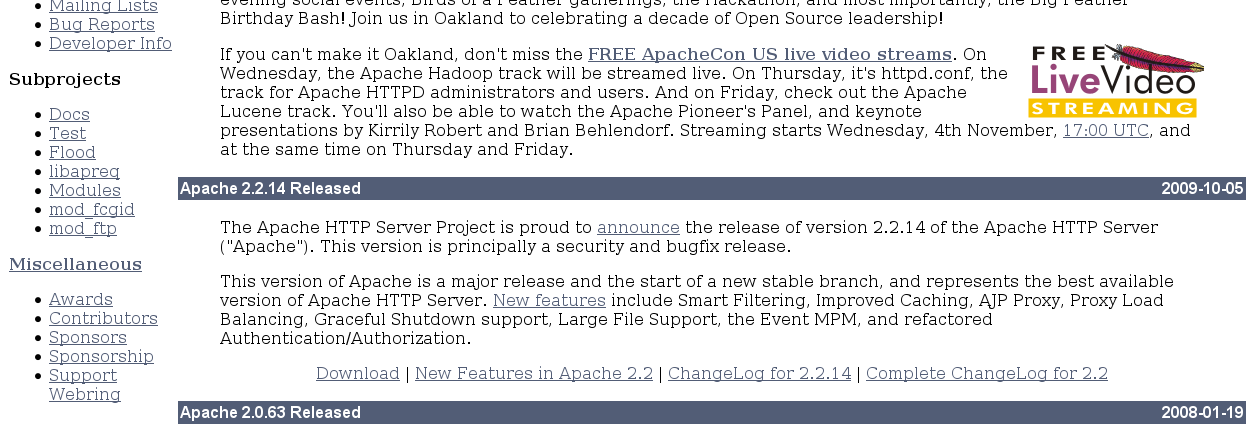
\includegraphics[width=400px]{cap01/Screenshot.png}
  \caption{Pagina oficială Apache HTTPD}
  \label{fig:httpd homepage}
\end{figure}


Alege un \textsl{mirror}\footnote{
Un mirror este o oglindire a unor fişiere. Mai multe firme sau instituţii au ales
să pună la dispoziţie oglindiri ale fişierelor de instalare pentru apache. Oricine
poate face un mirror, însă e recomandat să înştiinţezi autorul oficial, pentru
ca acesta să pună un link către mirror-ul tău. Toate fişierele de pe un mirror sunt identice,
deci teoretic nu contează ce mirror alegi, însă este recomandat să alegi un mirror
apropiat ţie din punct de vedere geografic, pentru ca descărcarea să fie mai
rapidă.} şi apasă \texttt{change}. Mirror-ul selectat automat ar trebui să fie unul
dintre cele mai bune. Apoi selectează versiunea {\glqq}Win32 Binary without crypto{\grqq}.

%\begin{figure}[h!]
%  \centering
%    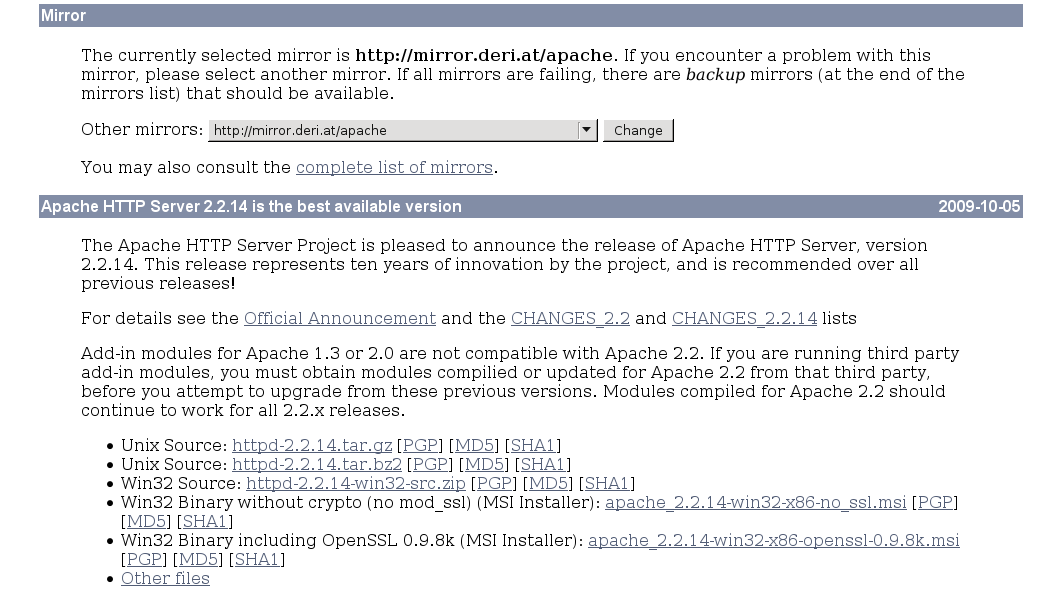
\includegraphics[width=400px]{cap01/Screenshot-1.png}
%  \caption{Setarea iniţială apache httpd}
%  \label{fig:httpd setup}
%\end{figure}

Introdu datele ca în figura \ref{fig:httpd setup} şi treci la pasul următor.

\begin{figure}[h!]
  \centering
    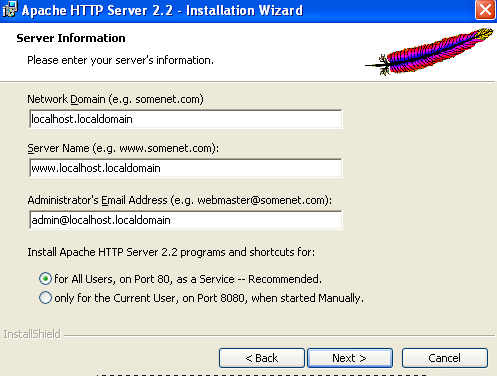
\includegraphics[width=300px]{cap01/Screenshot-2.png}
  \caption{Setarea iniţială apache httpd}
  \label{fig:httpd setup}
\end{figure}

Alege modul de instalare \texttt{custom}, deoarece vrem să decidem exact unde şi ce
se instalează, ca în \ref{fig:httpd check custom setup}.

\begin{figure}[h!]
  \centering
    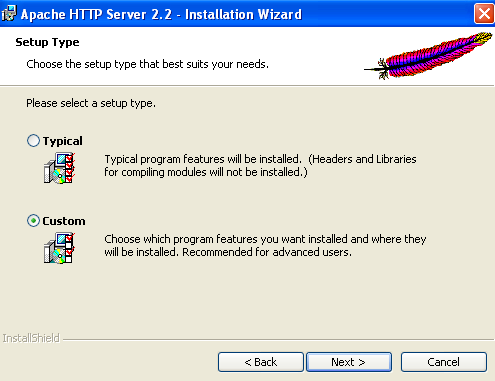
\includegraphics[width=250px]{cap01/Screenshot-3.png}
  \caption{Setare personalizată}
  \label{fig:httpd check custom setup}
\end{figure}

În figura \ref{fig:httpd components tree} avem un arbore cu toate componentele instalate. \texttt{Apache HTTP Server 2.2.14}
este părintele tuturor componentelor. Selectează-l şi apasă pe butonul
\texttt{Change...} pentru a schimba locul de instalare.

\begin{figure}[h!]
  \centering
    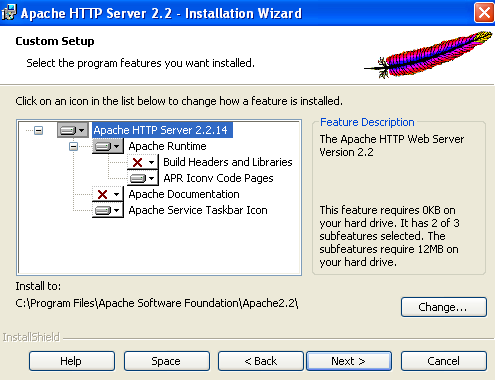
\includegraphics[width=248px]{cap01/Screenshot-4.png}
  \caption{Setare httpd - Componentele instalate}
  \label{fig:httpd components tree}
\end{figure}

Crează un nou director \texttt{C:{\textbackslash}webdev\textbackslash}
unde vor fi instalate toate sculele
de programare web, introducând manual calea \texttt{C:{\textbackslash}webdev{\textbackslash}apache}
exact ca în \ref{fig:httpd custom path}.

\begin{figure}[h!]
  \centering
    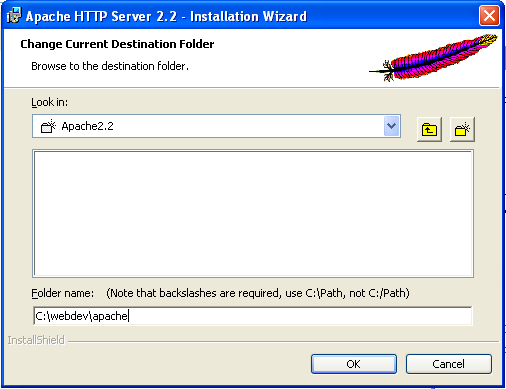
\includegraphics[width=253px]{cap01/Screenshot-5.png}
  \caption{Setare httpd - Calea instalării}
  \label{fig:httpd custom path}
\end{figure}

Confirmarea te va aduce la dialogul anterior, iar în partea de jos ar trebui să scrie
că programul va fi instalat la acea locaţie.

Finalizează instalarea. La vizitarea adresei \url{http://localhost/} ar trebui să
vezi mesajul \texttt{It works!}. Asta înseamnă că daemonul apache este setat corect şi poate deservi
pagini statice în formatul html, iar calculatorul tău este acum un server.

Noi însă vrem să generăm în mod dinamic cod HTML cu PHP. Deci intră pe pagina oficială
PHP\footnote{\url{http://php.net}} şi urmează linkul de download,
sub \texttt{Windows binaries} (Figura \ref{fig:php win bin}).

\attention{Toate programele care lucrează cu text, precum editoarele text şi browserele,
oferă o funcţionalitate de căutare a unui text. În majoritatea programelor, combinaţia
de taste \keystroke{CTRL+F} deschide un dialog de căutare. Fiind pe o pagină,
dacă nu găseşti un text, apasă această combinaţie de taste şi introdu titlurile
linkurilor sau orice alt text în a cărui căutare eşti.}

\begin{figure}[h!]
  \centering
    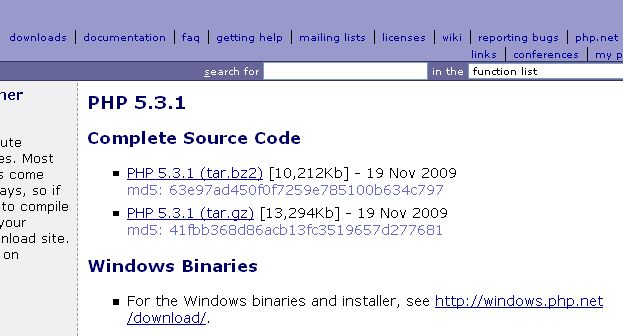
\includegraphics[width=340px]{cap01/Screenshot-6.png}
  \caption{PHP - Pagina oficială de download}
  \label{fig:php win bin}
\end{figure}

Selectează tipul de executabil \texttt{VC9 x86 Thread Safe} pentru
versiunea PHP 5.3, ca în \ref{fig:php build type}, apoi
descarcă arhiva .zip care conţine PHP, salvând-o în \texttt{C:{\textbackslash}webdev\textbackslash}.
\begin{figure}[h!]
  \centering
    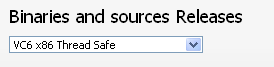
\includegraphics[width=150px]{cap01/Screenshot-7.png}
  \caption{PHP - Tipul \textsl{build}-ului PHP}
  \label{fig:php build type}
\end{figure}


%\begin{center}
%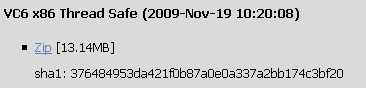
\includegraphics[width=200px]{cap01/Screenshot-8.png}
%\end{center}

După dezarhivare, conţinutul său va arăta ca în Figura \ref{fig:php what you get}.

\begin{figure}[h!]
  \centering
    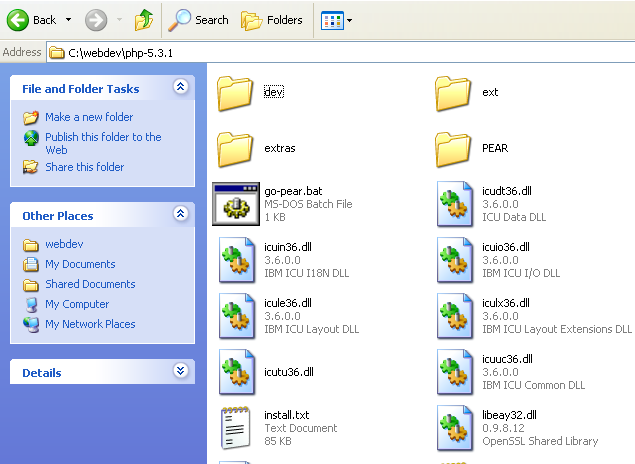
\includegraphics[width=200px]{cap01/Screenshot-9.png}
  \caption{PHP - What you get}
  \label{fig:php what you get}
\end{figure}

Înainte de a trece la integrarea lui PHP în apache, îţi recomand să
instalezi un editor text ideal pentru începătorii în programare:
\href{http://notepad-plus.sourceforge.net/}{Notepad++}
\footnote{\url{http://notepad-plus.sourceforge.net/}}, de pe pagina oficială.
%\begin{center}
%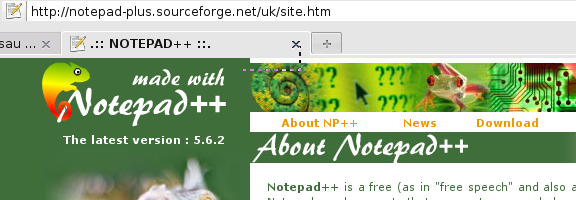
\includegraphics[width=320px]{cap01/Screenshot-10.png}
%\end{center}
%
%Descarcă programul de instalare şi instalează notepad++:
%\begin{center}
%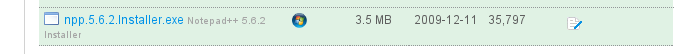
\includegraphics[width=350px]{cap01/Screenshot-11.png}
%\end{center}

\attention{Notepad++ este foarte bun ca editor deoarece, fiind un editor text,
vezi exact ce faci, preluând controlul, aşa cum ar trebui să o facă
orice programator. Pe lângă asta, Notepad++ îţi şi colorează textul
dacă recunoaşte limbajul în care scrii acel text, precum PHP sau HTML.}

\bad{Dacă eşti cumva tentat să foloseşti editoare WYSIWYG\footnote{what
you see is what you get} precum Dreamweaver, atunci ar trebui să
te opreşti acum - programarea nu e pentru tine. De ce? În afară
de faptul că un astfel de editor nu te-ar stimula să înveţi, ţi-ar
şi crea mai multe probleme. Cu PHP, tu ca programator vei prelua
controlul şi vei genera HTML. Pe lânga asta, astfel de programe
nu sunt destul de puternice ca o minte umană, şi mai şi generează
cod greşit.}
\footnotetext{\href{http://en.wikipedia.org/wiki/WYSIWYG}{what you see is what you get}}

PHP poate fi folosit şi ca limbaj de scripting general, nu doar pentru
generarea dinamică de HTML. Însă pentru asta trebuie setată calea
către directorul php care conţine fişierul de configurare \texttt{php.ini},
asupra căruia voi reveni puţin mai târziu.

Sub Windows XP, click dreapta pe \texttt{My Computer} şi apoi \texttt{Properties}.
Sub Windows 7, în \texttt{start} -> \texttt{run} introdu comanda:

\texttt{C:{\textbackslash}Windows{\textbackslash}System32{\textbackslash}SystemPropertiesAdvanced.exe}

Alege tabul \texttt{Advanced}, apoi click pe \texttt{Environment Variables} în partea de jos
a dialogului, aşa cum vezi în Figura \ref{fig:win adv props}.
\begin{figure}[h!]
  \centering
    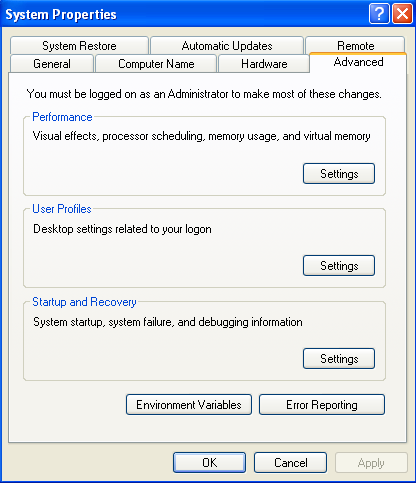
\includegraphics[width=200px]{cap01/Screenshot-12.png}
  \caption{Proprietăţile avansate ale sistemului Windows XP}
  \label{fig:win adv props}
\end{figure}

Se va deschide un dialog similar cu cel din Figura \ref{img:win env vars}.
\begin{figure}[h!]
  \centering
    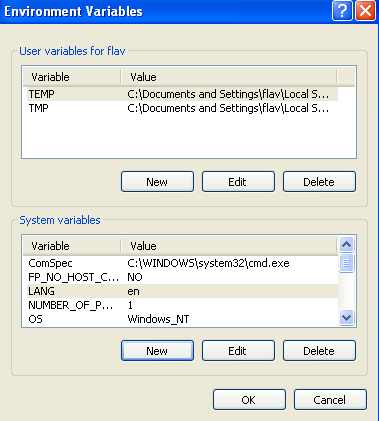
\includegraphics[width=180px]{cap01/Screenshot-13.png}
  \caption{Variabilele de mediu ale unui sistem Windows}
  \label{img:win env vars}
\end{figure}

Click pe \texttt{New} sub \texttt{System variables}, şi introdu datele ca în
Figura \ref{img:win new env var}. Această nouă variabilă de mediu
îl va ajuta pe PHP să-şi găsească fişierul de configurare \texttt{php.ini}.
\begin{figure}[h!]
  \centering
    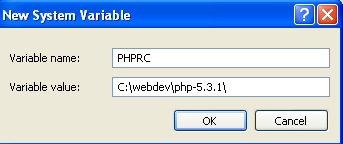
\includegraphics[width=180px]{cap01/Screenshot-14.png}
  \caption{Variabilele de mediu ale unui sistem Windows}
  \label{img:win new env var}
\end{figure}

În acest moment, PHP este setat şi l-am putea lansa în execuţie folosind
calea absolută
\texttt{C:{\textbackslash}webdev{\textbackslash}php-5.3.1{\textbackslash}php.exe}, ceea ce
poate deveni obositor cu timpul. Însă putem integra \texttt{php.exe}
în sistem astfel încât să fie recunoscut ca comandă.

Pentru ca asta să
se întâmple, identifică
variabila systemului numită \texttt{Path}
%\begin{figure}[h!]
%  \centering
%    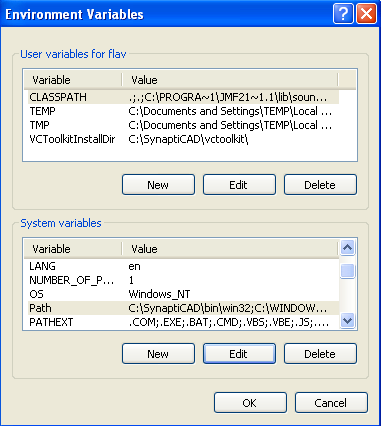
\includegraphics[width=180px]{cap01/Screenshot-20.png}
%  \caption{Variabila de mediu PATH}
%  \label{img:win env path}
%\end{figure}
şi adaugă-i la sfârşit:
\texttt{;C:{\textbackslash}webdev{\textbackslash}php-5.3.1{\textbackslash}}, ca în
Figura \ref{img:win env path}.
\begin{figure}[h!]
  \centering
    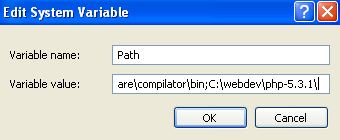
\includegraphics[width=180px]{cap01/Screenshot-21.png}
  \caption{Variabila de mediu PATH}
  \label{img:win env path}
\end{figure}

\attention{Acel ';' de la început este foarte important. \texttt{PATH}
conţine o listă de directoare în care windows se va uita pe rând atunci
când lansezi în execuţie un program ca pe o comandă. ';' are rolul
de a separa aceste directoare.}

Un singur lucru mai lipseşte: \texttt{php.ini}. Arhiva pe care tocmai
ai descărcat-o vine cu două astfel de fişiere, \texttt{php.ini-development} şi
\texttt{php.ini-production}. Fă o \textit{copie} a fişierului
\texttt{php.ini-development} şi redenumeşte-o \texttt{php.ini}.

Testează dacă ai setat totul cum trebuie deschizând o nouă instanţă
a promptului ms-dos.
Acolo introdu comanda \texttt{php --ini}.
Totul este corect dacă php este găsit de sistem, iar comanda de mai sus îţi
arată \texttt{C:{\textbackslash}webdev{\textbackslash}php-5.3.1{\textbackslash}php.ini}
ca \textit{Loaded Configuration File}.

%Mai multe informaţii despre PHP ca limbaj de scripting CLI găseşti pe
%\url{http://www.php-cli.com/}.

\vspace{1em}

Acum vom trece la integrarea lui PHP ca modul apache. Vom spune că folosim
\engl{SAPI-ul\footnote{\url{http://en.wikipedia.org/wiki/Server_Application_Programming_Interface}}}{server application programming interface}
apache2. În directorul în care ai instalat apache este un subdirector de configurare
numit sugestiv \texttt{conf/}, unde rezidă toate fişierele de configurare
pentru apache.

Fişierul principal de configurare  al apache se numeşte \texttt{httpd.conf}. Este singurul
fişier încărcat automat de apache pentru a citi configuraţia, celelalte fişiere
trebuie incluse folosind directiva \texttt{Include} din acest fişier
principal (en. \textsl{the master configuration file}). Liniile care încep
cu caracterul diez (\#) sunt comentarii, iar conţinutul lor nu este luat
în considerare, chiar dacă conţine directive de configurare valide.

Deschide \texttt{httpd.conf} cu notepad++ şi adaugă-i la sfârşit
(combinaţia \keystroke{CTRL+END}) directiva
\texttt{Include conf/extra/httpd-php.conf}
apoi crează un nou fişier cu \keystroke{CTRL+N} cu acest conţinut:
\begin{verbatim}
LoadModule php5_module "C:/webdev/php-5.3.1/php5apache2_2.dll"
AddType application/x-httpd-php .php
PHPIniDir "C:/webdev/php-5.3.1"

<IfModule dir_module>
    DirectoryIndex index.php index.html
</IfModule>
\end{verbatim}

Acum apasă \keystroke{CTRL+S} şi salvează-l ca \texttt{httpd-php.conf}
în directorul
C:\texttt{{\textbackslash}webdev{\textbackslash}apache{\textbackslash}conf{\textbackslash}extra{\textbackslash}}

Directiva \texttt{LoadModule} îi spune să încarce un fişier ca modul apache. \texttt{AddType}
îl instruieşte să interpreteze fişiere ce se termină în .php ca 
\texttt{application/x-httpd-php}, care este un tip 
\engl{MIME\footnote{\url{http://en.wikipedia.org/wiki/Multipurpose_Internet_Mail_Extensions}}}{multipurpose internet mail extension}.
\texttt{PHPIniDir} îi spune lui PHP (de data asta modulului PHP) unde îşi găseşte fişierul
de configurare \texttt{php.ini}, aşa cum variabila de mediu \texttt{PHPRC} pe care
am setat-o anterior îi spune acelaşi lucru SAPI-ului CLI (adică lui \texttt{php.exe}).

Acel bloc condiţional\footnote{Se numeşte condiţional deoarece ceea ce se află
în interiorul său este inclus doar dacă condiţia este adevărată, numele însuşi
conţinând \texttt{If}.}
 \texttt{IfModule} verifică dacă apache are modulul {\glqq}dir{\grqq}, şi dacă
da, setează resursa de start corespunzătoare root-ului (atunci când este accesat {\glqq}/{\grqq}
al unui director, aşa cum ai văzut în capitolul anterior) fiecărui director. Fişierele
sunt listate după ordinea priorităţii, dacă primul nu este găsit, apache va încerca să-l
deservească pe al doilea.

\attention{O altă directivă importantă din \texttt{httpd.conf} este
\texttt{DocumentRoot}. Acesta îi spune lui apache de unde
să deservească fişiere. În mod standard, acest director se numeşte
\texttt{htdocs} -- \textsl{hypertext documents}.}

Acum că avem totul setat, restartează daemonul httpd, în caz că e pornit, pentru a prelua
toate schimbările din \texttt{httpd.conf} şi fişierele incluse de acesta. Ar fi trebuit să-i
dăm restart şi dacă am fi modificat configuraţia php din \texttt{php.ini}.

Pentru a verifica instalarea şi configurarea lui PHP ca modul apache, crează un nou fişier
şi salvează-l ca 
\texttt{C:{\textbackslash}webdev{\textbackslash}apache{\textbackslash}htdocs{\textbackslash}info.php}
. Apoi introdu următorul text, numit şi cod sursă (în limbajul PHP):
\lstinputlisting[caption={phpinfo() furnizează toate informaţiile despre instalarea PHP curentă}]{cap01/info.php}
şi salvează-l. 

Acum intră pe adresa \url{http://localhost/info.php}. Ar trebui să vezi ceva similar cu Figura \ref{img:php phpinfo}.

\begin{figure}[h!]
  \centering
    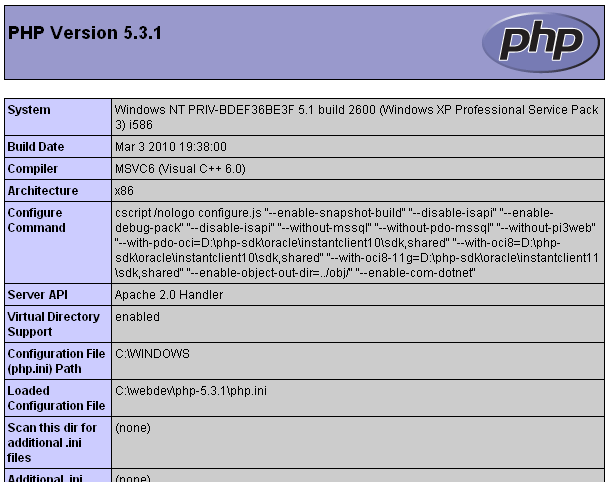
\includegraphics[width=300px]{cap01/Screenshot-15.png}
  \caption{Informaţii afişate de un apel la phpinfo()}
  \label{img:php phpinfo}
\end{figure}

Felicitări, acum ai PHP instalat şi poţi învăţa programare, fie folosindu-l pentru programare web
ca modul apache, fie folosindu-l ca limbaj de scripting universal folosind SAPI-ul CLI (programul \texttt{php.exe}).

SAPI-urile există tocmai pentru a uşura integrarea lui PHP în toate aceste medii: pentru web putem folosi
un SAPI specific daemonului folosit, de exemplu pentru apache avem SAPI-ul php5apache2\_2.dll.
Acest fişier DLL reprezintă însă doar interfaţa (SAPI-ul, aşa cum îi spune şi numele de \textsl{interface})
de comunicare dintre apache şi "adevăratul PHP".

Pe acelaşi calapod, \texttt{php.exe} reprezintă interfaţa de comunicare dintre promptul ms-dos
(sau shell, într-un sistem *NIX) şi acelaşi "adevărat PHP" ca şi în cazul apache. Altfel spus,
ambele, atât \texttt{php.exe}, cât şi \texttt{php5apache2\_2.dll} sunt două SAPI-uri,
fiecare destinate integrării lui PHP în mediile lor specifice de execuţie a scripturilor PHP.

În capitolul următor ne vom uita mai îndeaproape la limbajul PHP.
